\documentclass{standalone}
\usepackage{tikz}
\usetikzlibrary{patterns, positioning}
\usepackage[sfdefault]{ClearSans} %% option 'sfdefault' activates Clear Sans as the default text font
\usepackage[T1]{fontenc}

\begin{document}
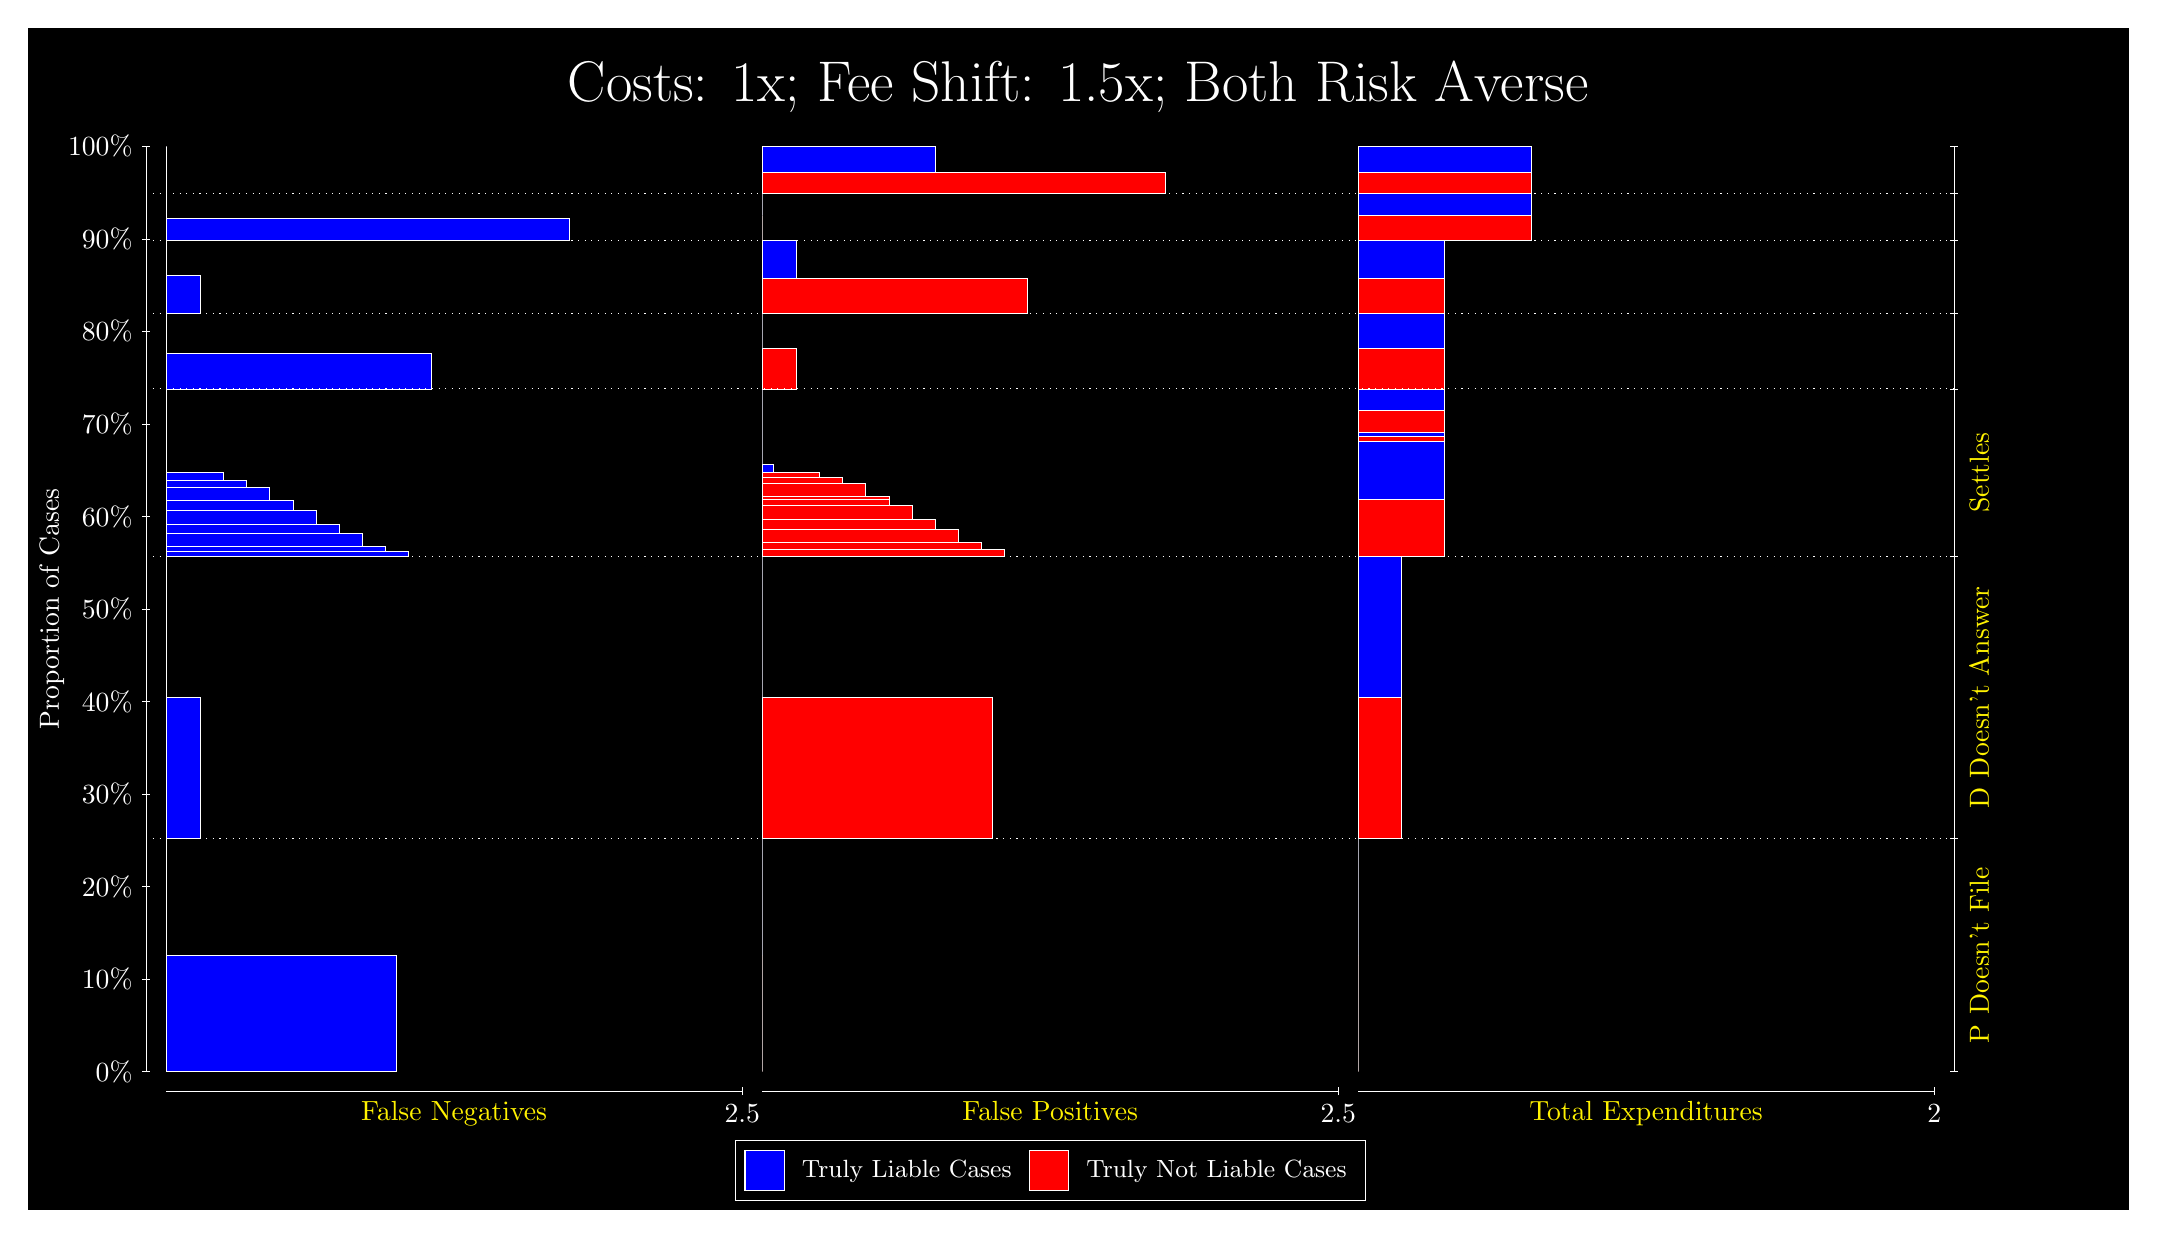
\begin{tikzpicture}
\draw[fill=black] (0,0) rectangle (26.667,15);
\draw[text=white] (0,13.5) rectangle (26.667,15) node[midway] {\huge Costs: 1x; Fee Shift: 1.5x; Both Risk Averse};
\draw[white, very thin] (1.5,1.75) -- (1.5,13.5);
\node[rotate=90, text=white, anchor=center] at (0.3, 7.625) {Proportion of Cases};
\draw[white, very thin] (1.45,1.75) -- (1.55,1.75);
\node[text=white, anchor=east] at (1.45, 1.75) {0\%};
\draw[white, very thin] (1.45,2.925) -- (1.55,2.925);
\node[text=white, anchor=east] at (1.45, 2.925) {10\%};
\draw[white, very thin] (1.45,4.1) -- (1.55,4.1);
\node[text=white, anchor=east] at (1.45, 4.1) {20\%};
\draw[white, very thin] (1.45,5.275) -- (1.55,5.275);
\node[text=white, anchor=east] at (1.45, 5.275) {30\%};
\draw[white, very thin] (1.45,6.45) -- (1.55,6.45);
\node[text=white, anchor=east] at (1.45, 6.45) {40\%};
\draw[white, very thin] (1.45,7.625) -- (1.55,7.625);
\node[text=white, anchor=east] at (1.45, 7.625) {50\%};
\draw[white, very thin] (1.45,8.8) -- (1.55,8.8);
\node[text=white, anchor=east] at (1.45, 8.8) {60\%};
\draw[white, very thin] (1.45,9.975) -- (1.55,9.975);
\node[text=white, anchor=east] at (1.45, 9.975) {70\%};
\draw[white, very thin] (1.45,11.15) -- (1.55,11.15);
\node[text=white, anchor=east] at (1.45, 11.15) {80\%};
\draw[white, very thin] (1.45,12.325) -- (1.55,12.325);
\node[text=white, anchor=east] at (1.45, 12.325) {90\%};
\draw[white, very thin] (1.45,13.5) -- (1.55,13.5);
\node[text=white, anchor=east] at (1.45, 13.5) {100\%};

\draw[white, very thin] (24.457,1.75) -- (24.457,13.5);
\draw[white, very thin] (24.407,1.75) -- (24.507,1.75);
\node[anchor=west] at (24.407, 1.75) {};
\draw[white, very thin] (24.407,4.7064) -- (24.507,4.7064);
\node[anchor=west] at (24.407, 4.7064) {};
\draw[white, very thin] (24.407,8.2946) -- (24.507,8.2946);
\node[anchor=west] at (24.407, 8.2946) {};
\draw[white, very thin] (24.407,10.419) -- (24.507,10.419);
\node[anchor=west] at (24.407, 10.419) {};
\draw[white, very thin] (24.407,11.381) -- (24.507,11.381);
\node[anchor=west] at (24.407, 11.381) {};
\draw[white, very thin] (24.407,12.305) -- (24.507,12.305);
\node[anchor=west] at (24.407, 12.305) {};
\draw[white, very thin] (24.407,12.901) -- (24.507,12.901);
\node[anchor=west] at (24.407, 12.901) {};
\draw[white, very thin] (24.407,13.5) -- (24.507,13.5);
\node[anchor=west] at (24.407, 13.5) {};

\draw[white, very thin, fill=blue] (1.75,1.75) rectangle (4.6775,3.2282);
\draw[white, very thin, fill=red] (1.75,3.2282) rectangle (1.75,4.7064);
\draw[white, very thin, fill=blue] (1.75,4.7064) rectangle (2.1891,6.5005);
\draw[white, very thin, fill=red] (1.75,6.5005) rectangle (1.75,8.2946);
\draw[white, very thin, fill=blue] (1.75,8.2946) rectangle (4.8239,8.3551);
\draw[white, very thin, fill=blue] (1.75,8.3551) rectangle (4.5312,8.4261);
\draw[white, very thin, fill=blue] (1.75,8.4261) rectangle (4.2384,8.5853);
\draw[white, very thin, fill=blue] (1.75,8.5853) rectangle (3.9457,8.6964);
\draw[white, very thin, fill=blue] (1.75,8.6964) rectangle (3.6529,8.8749);
\draw[white, very thin, fill=blue] (1.75,8.8749) rectangle (3.3602,9.0008);
\draw[white, very thin, fill=blue] (1.75,9.0008) rectangle (3.0674,9.1694);
\draw[white, very thin, fill=blue] (1.75,9.1694) rectangle (2.7746,9.254);
\draw[white, very thin, fill=blue] (1.75,9.254) rectangle (2.4819,9.3555);
\draw[white, very thin, fill=red] (1.75,9.3555) rectangle (1.75,10.419);
\draw[white, very thin, fill=blue] (1.75,10.419) rectangle (5.1167,10.868);
\draw[white, very thin, fill=red] (1.75,10.868) rectangle (1.75,11.381);
\draw[white, very thin, fill=blue] (1.75,11.381) rectangle (2.1891,11.865);
\draw[white, very thin, fill=red] (1.75,11.865) rectangle (1.75,12.305);
\draw[white, very thin, fill=blue] (1.75,12.305) rectangle (6.8732,12.584);
\draw[white, very thin, fill=red] (1.75,12.584) rectangle (1.75,12.901);
\draw[white, very thin, fill=red] (1.75,12.901) rectangle (1.75,13.171);
\draw[white, very thin, fill=blue] (1.75,13.171) rectangle (1.75,13.5);
\draw[white, very thin, fill=red] (9.3189,1.75) rectangle (9.3189,3.2282);
\draw[white, very thin, fill=blue] (9.3189,3.2282) rectangle (9.3189,4.7064);
\draw[white, very thin, fill=red] (9.3189,4.7064) rectangle (12.246,6.5005);
\draw[white, very thin, fill=blue] (9.3189,6.5005) rectangle (9.3189,8.2946);
\draw[white, very thin, fill=red] (9.3189,8.2946) rectangle (12.393,8.3876);
\draw[white, very thin, fill=red] (9.3189,8.3876) rectangle (12.1,8.4726);
\draw[white, very thin, fill=red] (9.3189,8.4726) rectangle (11.807,8.639);
\draw[white, very thin, fill=red] (9.3189,8.639) rectangle (11.515,8.7643);
\draw[white, very thin, fill=red] (9.3189,8.7643) rectangle (11.222,8.9442);
\draw[white, very thin, fill=red] (9.3189,8.9442) rectangle (10.929,9.0178);
\draw[white, very thin, fill=red] (9.3189,9.0178) rectangle (10.929,9.0571);
\draw[white, very thin, fill=red] (9.3189,9.0571) rectangle (10.636,9.2204);
\draw[white, very thin, fill=red] (9.3189,9.2204) rectangle (10.344,9.2922);
\draw[white, very thin, fill=red] (9.3189,9.2922) rectangle (10.051,9.3582);
\draw[white, very thin, fill=blue] (9.3189,9.3582) rectangle (9.4652,9.4597);
\draw[white, very thin, fill=blue] (9.3189,9.4597) rectangle (9.3189,10.419);
\draw[white, very thin, fill=red] (9.3189,10.419) rectangle (9.758,10.932);
\draw[white, very thin, fill=blue] (9.3189,10.932) rectangle (9.3189,11.381);
\draw[white, very thin, fill=red] (9.3189,11.381) rectangle (12.686,11.82);
\draw[white, very thin, fill=blue] (9.3189,11.82) rectangle (9.758,12.305);
\draw[white, very thin, fill=red] (9.3189,12.305) rectangle (9.3189,12.622);
\draw[white, very thin, fill=blue] (9.3189,12.622) rectangle (9.3189,12.901);
\draw[white, very thin, fill=red] (9.3189,12.901) rectangle (14.442,13.171);
\draw[white, very thin, fill=blue] (9.3189,13.171) rectangle (11.515,13.5);
\draw[white, very thin, fill=red] (16.888,1.75) rectangle (16.888,3.2282);
\draw[white, very thin, fill=blue] (16.888,3.2282) rectangle (16.888,4.7064);
\draw[white, very thin, fill=red] (16.888,4.7064) rectangle (17.437,6.5005);
\draw[white, very thin, fill=blue] (16.888,6.5005) rectangle (17.437,8.2946);
\draw[white, very thin, fill=red] (16.888,8.2946) rectangle (17.986,9.0178);
\draw[white, very thin, fill=blue] (16.888,9.0178) rectangle (17.986,9.7478);
\draw[white, very thin, fill=red] (16.888,9.7478) rectangle (17.986,9.8138);
\draw[white, very thin, fill=blue] (16.888,9.8138) rectangle (17.986,9.8743);
\draw[white, very thin, fill=red] (16.888,9.8743) rectangle (17.986,10.149);
\draw[white, very thin, fill=blue] (16.888,10.149) rectangle (17.986,10.419);
\draw[white, very thin, fill=red] (16.888,10.419) rectangle (17.986,10.932);
\draw[white, very thin, fill=blue] (16.888,10.932) rectangle (17.986,11.381);
\draw[white, very thin, fill=red] (16.888,11.381) rectangle (17.986,11.82);
\draw[white, very thin, fill=blue] (16.888,11.82) rectangle (17.986,12.305);
\draw[white, very thin, fill=red] (16.888,12.305) rectangle (19.083,12.622);
\draw[white, very thin, fill=blue] (16.888,12.622) rectangle (19.083,12.901);
\draw[white, very thin, fill=red] (16.888,12.901) rectangle (19.083,13.171);
\draw[white, very thin, fill=blue] (16.888,13.171) rectangle (19.083,13.5);
\draw[white, dotted] (1.5,4.7064) -- (24.457,4.7064);
\draw[white, dotted] (1.5,8.2946) -- (24.457,8.2946);
\draw[white, dotted] (1.5,10.419) -- (24.457,10.419);
\draw[white, dotted] (1.5,11.381) -- (24.457,11.381);
\draw[white, dotted] (1.5,12.305) -- (24.457,12.305);
\draw[white, dotted] (1.5,12.901) -- (24.457,12.901);
\draw[white, very thin] (1.75,1.5) -- (9.0689,1.5);
\node[text=yellow, anchor=north] at (5.4094, 1.5) {False Negatives};
\draw[white, very thin] (9.0689,1.45) -- (9.0689,1.55);
\node[text=white, anchor=north] at (9.0689, 1.45) {2.5};

\draw[white, very thin] (9.3189,1.5) -- (16.638,1.5);
\node[text=yellow, anchor=north] at (12.978, 1.5) {False Positives};
\draw[white, very thin] (16.638,1.45) -- (16.638,1.55);
\node[text=white, anchor=north] at (16.638, 1.45) {2.5};

\draw[white, very thin] (16.888,1.5) -- (24.207,1.5);
\node[text=yellow, anchor=north] at (20.547, 1.5) {Total Expenditures};
\draw[white, very thin] (24.207,1.45) -- (24.207,1.55);
\node[text=white, anchor=north] at (24.207, 1.45) {2};

\node[text=yellow, centered, rotate=90] at (24.777, 3.2282) {P Doesn't File};
\node[text=yellow, centered, rotate=90] at (24.777, 6.5005) {D Doesn't Answer};
\node[text=yellow, centered, rotate=90] at (24.777, 9.3568) {Settles};





\draw (12.978300999999998,1.5) node[draw=none] (baseCoordinate) {};
\begin{scope}[align=center]
        \matrix[scale=0.5, draw=white, below=0.5cm of baseCoordinate, nodes={draw}, column sep=0.1cm]{
            \node[rectangle, draw, minimum width=0.5cm, minimum height=0.5cm, fill=blue] {}; &
            \node[draw=none, font=\small, text=white] (B) {Truly Liable Cases}; &
            \node[rectangle, draw, minimum width=0.5cm, minimum height=0.5cm, fill=red] {}; &
            \node[draw=none, font=\small, text=white] (B) {Truly Not Liable Cases}; \\
            };
\end{scope}

\end{tikzpicture}
\end{document}